\section{Channel Controls}

As shown in \cref{fig:09-four-channels}, four identical groups of ``channel'' controls are positioned to the left of the main animation window. \cref{fig:09-single-channel} zooms in one of them, whose individual settings are explained next.

\begin{figure}
    \centering
    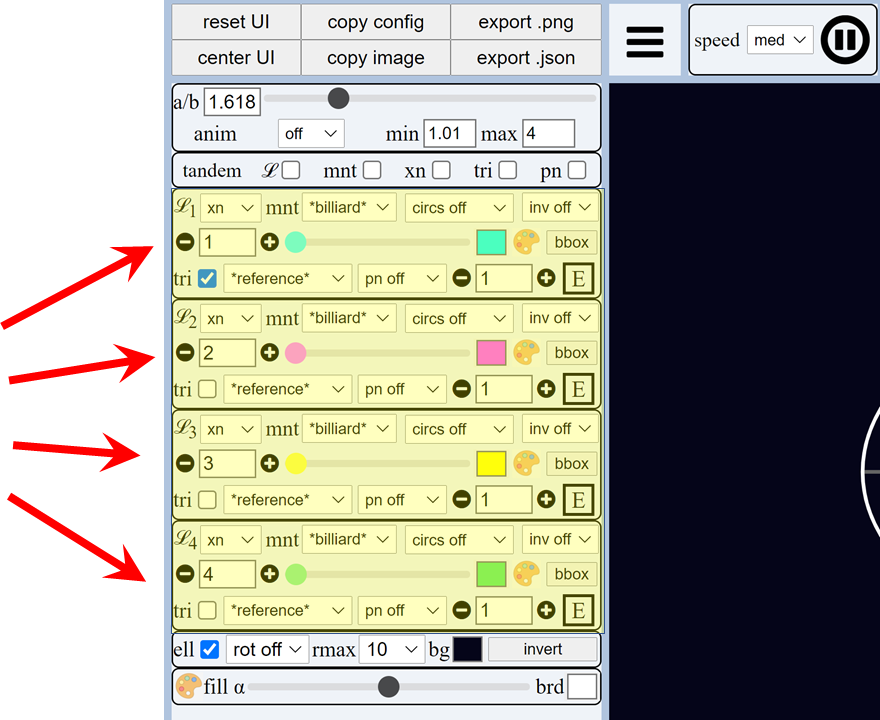
\includegraphics[width=.6\textwidth]{pics_09_030_four_channels.png}
    \caption{Four identical groups of ``channel'' controls positioned to theleft of the main animation window.}
    \label{fig:09-four-channels}
\end{figure}

%\includegraphics[trim=left bottom right top, clip]
\begin{figure}
    \centering
    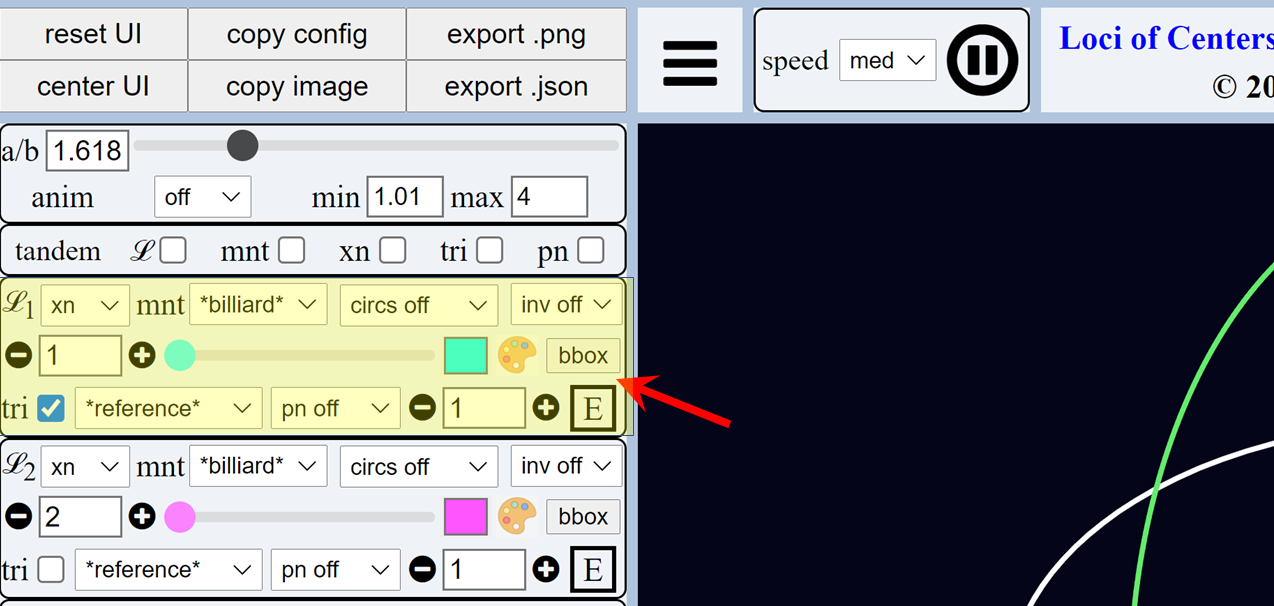
\includegraphics[trim=0 0 150 0,clip,width=.6\textwidth]{pics_09_040_single_channel.png}
    \caption{Various settings in a single channel control.}
    \label{fig:09-single-channel}
\end{figure}

\section{Choosing a triangle family}

The first step in \cref{fig:09-flow} is the choice of a triangle {\em family}. A specific one is selected 
via the \texttt{mnt} drop-down, see \cref{fig:09-menu-family}. Two types of families are supported: (i) Poncelet, and (ii) ellipse ``mounted'' (see below), which originated the name of the control.

\begin{figure}
    \centering
    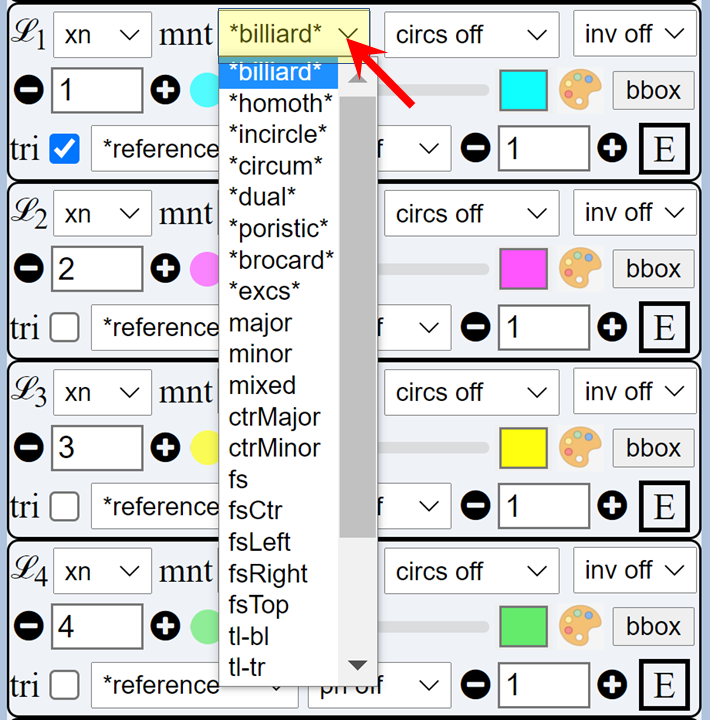
\includegraphics[width=.6\textwidth]{pics_09_050_family.png}
    \caption{The \texttt{mnt} drop-down selects a triangle family.}
    \label{fig:09-menu-family}
\end{figure}

\subsection{Poncelet families} Currently we support the following 8 types of 3-periodic Poncelet families interscribed between axis-parallel ellipses, whose names are familiar from previous sections: (i) Confocal (i.e., elliptic billiard), (ii) Homothetic, (iii) with Incircle, (iv) with Circumcircle, (v) Dual, (vi) Excentral (to confocals),  (vii) Poristic, and (viii) the Brocard Porism. Note (i)-(vi),  while the last two are non-concentric.

\subsection{Ellipse ``Mounted''}

Also selectable are triangle families $\T(t)=V_1 V_2 P(t)$, where $V_1,V_2$ are pinned to two points on or near an ellipse, and $P(t)=[a\cos{t},b\sin{t}]$ sweeps the boundary. Let The following fixed locations for $V_1$ and $V_2$ are currently supported:

\begin{enumerate}
    \item \texttt{major}: left and right ellipse vertices (EVs)
    \item \texttt{minor}: top and bottom EVs
    \item \texttt{mixed}: left and top EVs
    \item \texttt{ctrMajor}: center and left EV
    \item \texttt{ctrMinor}: center and top EV 
    \item \texttt{fs}: the 2 foci $f_1$ and $f_2$
    \item \texttt{fsCtr}: center and right focus ($f_2$)
    \item \texttt{fsLeft}: left EV and $f_2$
    \item \texttt{fsRight}: right EV and $f_2$
    \item \texttt{fsTop}: top EV and $f_2$
    \item \texttt{tl-bl}: top left corner of ellipse bounding box (TL) and bottom left of the same (BL)
    \item \texttt{tl-tr}: TL and top right corner (TR) of ellipse bounding box
    \item \texttt{tl-l}: TL and left EV
    \item \texttt{tl-t}: TL and top EV
    \item \texttt{tl-b}: TL and bottom EV
    \item \texttt{tl-o}: TL and center of ellipse
    \item \texttt{tl-br}: TL and center of ellipse
\end{enumerate}

\section{Triangle Type}
\label{sec:09-triangle-type}

The second step in \cref{fig:09-flow} is the choice of the type of triangle with respect to which centers and loci will be computed. This is done the \texttt{tri}  checkbox and drop-down, as shown in \cref{fig:09-menu-triangle}.

\begin{figure}
    \centering
    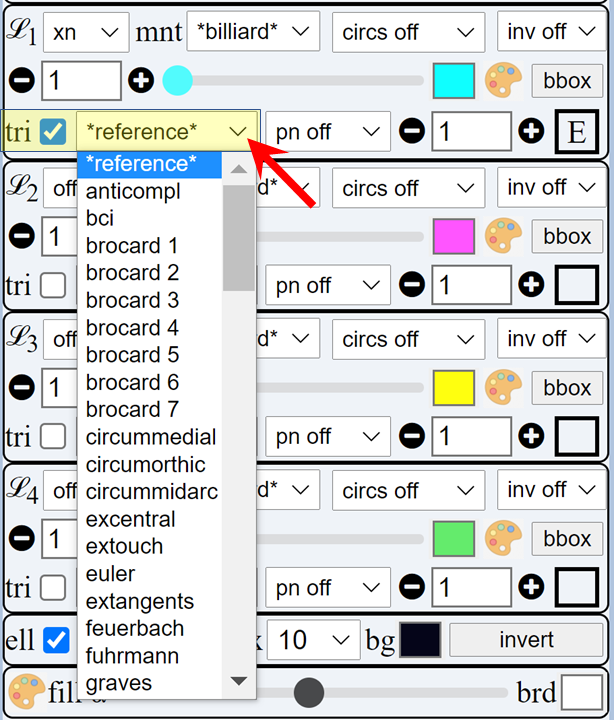
\includegraphics[width=.6\textwidth]{pics_09_060_triangle.png}
    \caption{The triangle menu selects whether a \texttt{*reference*} or some derived triangle should be used to compute loci. The \texttt{tri} checkbox immediate to the left selects whether the triangle should be drawn or not.}
    \label{fig:09-menu-triangle}
\end{figure}

While the checkbox controls whether selected triangle is drawn or not, the drop-down contains some four-dozen derived triangles. Below the default setting \texttt{*reference*} (this indicates a plain triangle in the family should be used), the choices are organized in three groups:

\begin{enumerate}
    \item Standard ``named'' triangles (undecorated abbreviations), such as \texttt{anticompl} for anticomplementary, \texttt{bci} for BCI triangle, etc., whose construction can be looked up in \cite{mw}.
    \item Exotic triangles (prefixed by a ``.''): \texttt{.andromeda}, \texttt{.antlia}, etc., obtained from \cite{lozada2016-triangles}.
    \item Inversive triangles, e.g., \texttt{*inv-f1*}, \texttt{*inv-f1c*}, etc. (decorated with asterisks). 
\end{enumerate}

Below we document triangles both in the ``standard'' and ``exotic'' groups:

\subsection{Standard Triangles}

These include: Reference, Anticomplementary, BCI, 1st Brocard, 2nd Brocard, 3rd Brocard, 4th Brocard, 5th Brocard, 6th Brocard, 7th Brocard, Circum-Medial, Circum-Mid-arc, Circum-Orthic, Excentral, Extouch, Extangents, Feuerbach, Fuhrmann, Half-Altitude, Hexyl, Incentral, Inner Vecten, Intangents, Intouch, Johnson, Lemoine, Lucas Central, Lucas Inner, Lucas Tangents, MacBeath, Medial, Mixtilinear, 1st Morley Adj, 2nd Morley Adj, 3rd Morley Adj, 1st Neuberg, 2nd Neuberg, Orthic, Outer Vecten, Reflection, Steiner, Symmedial, Tangential, Tangential Mid-Arc, Yff Central, Yff Contact.

\subsection{Exotic Triangles}

These include: Andromeda, Antlia, Apollonius, Apus, Atik, Ayme, Bevan-Antipodal, 1st Circumperp, 2nd Circumperp, Excenters-Incenter Reflections, Excenters-Midpoints, Honsberger, Inverse-in-Excircles, Inverse-in-Incircle, Kosnita, Mandart Excircles, Mandart Incircles, Ursa Major, Ursa Minor. 

\subsection{Inversive Triangles}
\label{sec:09-adv-tri-families}

The options below are images of the reference triangle in a given family under an inversive-like transformation with respect to  unit circle centered on a stationary notable point of the family's underlying ellipse (or caustic), e.g., center, focus, etc.

\begin{itemize}
\item \texttt{*inv-ctr*,*inv-f1*,*inv-f1c*,*inv-f2*}: inversion of vertices with respect to a unit circle centered on the outer ellipse center, outer ellipse left focus, inner ellipse left focus, or outer ellipse right focus, respectively.
\item \texttt{*pol-ctr*,*pol-f1*,*pol-f1c*}: a new, ``polar'' triangle is computed bounded by the polars of the vertices with respect to ellipse center, outer ellipse left focus, or inner ellipse left focus, respectively.
\item \texttt{*ped-lim2*}: this is specific to the confocal family. Computes the pedal triangle with respect to the non-focal limiting point of the bicentric family which is the polar image of the confocal family. 
\item \texttt{*x3map-ctr*,*x3map-f1*,*x3map-f1c*}: consider a triangulation of the original triangle in 3 subtriangles, each of which contains two vertices of the original triangle and either (i) the center of the outer ellipse, (ii) its left focus, or (iii) the inner ellipse left focus, respectively. These transformations compute a new triangle with vertices at the circumcenter of each subtriangle.
\item \texttt{*x3inv-ctr*,*x3inv-f1*,*x3inv-f1c*}: these compute the inverses of the previous transform with respect to the same points.
\item \texttt{*crem-ctr*,*crem-f1*,*crem-f2*}: sends the reference vertices to their images under a quadratic Cremona transformation, which sends $(x,y)\rightarrow(1/x,1/y)$. The origin will be the center of the outer ellipse, its left focus, or its right focus, respectively. 
\end{itemize}

Note: four additional settings \texttt{*inf-x*,*inf-y*,*inf-x2*,*inf-y2*} are provided and are experimental and non-inversive. They dynamically set the $x$ or $y$ coordinate of each vertex so they slide along infinity-like Lissajous curves. 

\section{Locus Type}

The third step in \cref{fig:09-flow} is the choice of type of locus to be drawn, or more precisely, the feature selected from the family/triangle combination previously selected. This is done with the $\mathcal{L}_i$ menu at the top of the control group, $i=1,2,3,4$, shown in \cref{fig:09-menu-locus}.

\begin{figure}
    \centering
    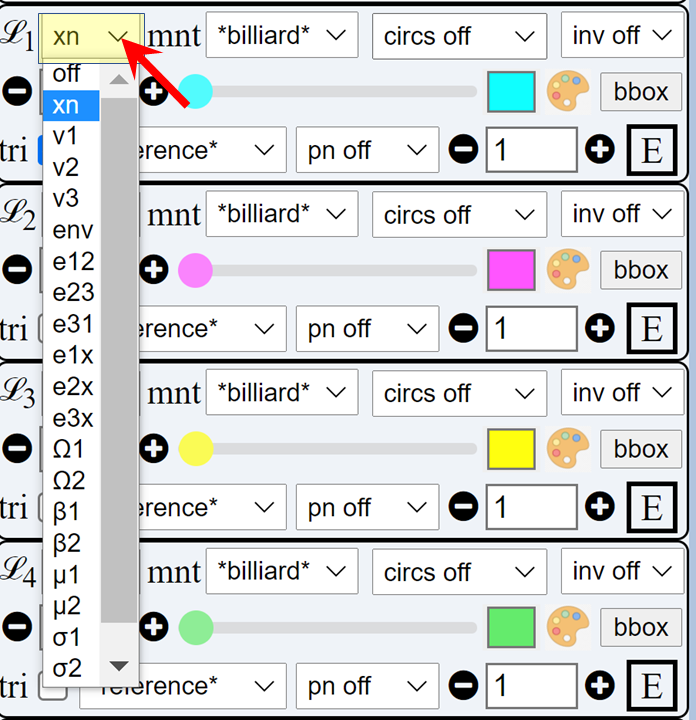
\includegraphics[width=.6\textwidth]{pics_09_070_locus.png}
    \caption{The $\mathcal{L}_i$ menu selects the locus type to (triangle center, vertex, envelope, etc.).}
    \label{fig:09-menu-locus}
\end{figure}

There are three conceptual groups of locus types: (i) triangle centers and vertices, (ii) segment envelopes, and (iii) bicentric pairs. These are explained next.

\subsection{Centers and Vertices}

\begin{enumerate}
\item \texttt{off}: it indicates the trace (locus) of this channel should not be drawn. It is the default setting for channels $2,3,4$ upon startup.
\item \texttt{xn}: draw the locus of the selected triangle center, as in  \cref{sec:09-triangle-center};
\item \texttt{v1}, \texttt{v2}, \texttt{v3}: show the trace of one of thee vertices of the triangle family. In Poncelet families, these will sweep out the same curve, but this is not the case for ellipse-mounted families.
\item \texttt{ort}: the {\em orthopole} of line $X_m X_n$, see \cite[Orthopole]{mw}, where $m$ and $n$ are selected triangle and cevian centers, see \cref{sec:09-triangle-center} and \cref{sec:09-cevian}.
\end{enumerate}

\subsection{Envelopes}

\begin{enumerate}
\item \texttt{env}: the envelope of segment $X_m X_n$, $m{\neq}n$, where $m$ (resp. $n$) is the selected triangle (resp. cevian) center. 
\item \texttt{e12}, \texttt{e23}, \texttt{e31}: the envelope of side $V_i V_j$ of the triangle family. Note these are one and the same (resp. distinct) for Poncelet (ellipse-mounted) families. 
\item \texttt{e1x}, \texttt{e2x}, \texttt{e3x}: the envelope of $V_i X_n$, i.e., the line from a given vertex to a selected triangle center. In a concentric Poncelet family, the envelope of $V_i X_1$ will be the outer ellipse's evolute, see it \href{https://bit.ly/3fNKV2P}{Live}.
\end{enumerate}

\subsection{Bicentric Pairs}

Only a few have so far been implemented, from the copious list in \cite{kimberling2020-bicentric}.

\begin{enumerate}
 \item $\Omega_1,\Omega_2$: the Brocard points
    \item $\beta_1,\beta_2$: the Beltrami points: inversions of the Brocard points with respect to the circumcircle
    \item $\mu_1,\mu_2$: also known as ``Moses'' points: inversion of the Brocard points with respect to the incircle.
    \item $\sigma_1,\sigma_2$: the two foci of the Steiner circumellipse (aka. the Bickart points)
\end{enumerate}

\section{Triangle Center}
\label{sec:09-triangle-center}

The fourth and final step in \cref{fig:09-flow} is the choice of triangle center $X_k$ in the region highlighted in \cref{fig:09-menu-xn}. There are three ways to choose $k\in[1,1000]$: (i) by typing/editing the text field showing $k$, (ii) incrementing or decrementing $k$ by clicking on the ``-'' and ``+'' symbols around the text field; (iii) using the scrollbar to the right of the ``+'' control, to quickly scroll through all 1000 values of $k$. In fact after any of these is performed, this set of controls becomes ``focused'' in such a way that (iv) left (resp. right) arrow keystrokes will decrement (resp. increment) the value, allowing mouse-free traversal of triangle centers.

\begin{figure}
    \centering
    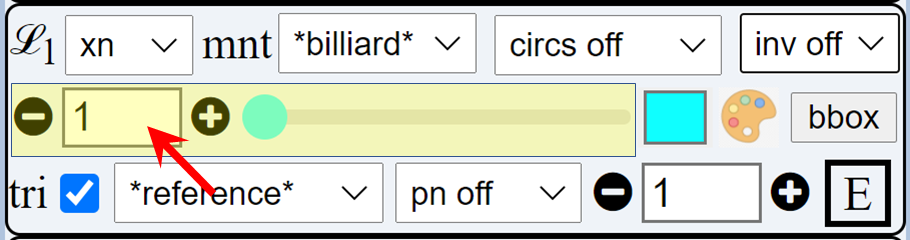
\includegraphics[width=.6\textwidth]{pics_09_080_xn.png}
    \caption{Controls used for the selection of a particular triangle center $X_k$.}
    \label{fig:09-menu-xn}
\end{figure}


